\documentclass[tikz,border=7pt]{standalone}

\usepackage{amsmath}
\usetikzlibrary{arrows.meta,calc,fit,positioning}

\definecolor{fixedblue}{HTML}{4C78A8}
\definecolor{weatherorange}{HTML}{F28E2B}
\definecolor{rnnpurple}{HTML}{8B6BB1}
\definecolor{outputgreen}{HTML}{59A14F}
\definecolor{inputrose}{HTML}{C46A75}
\definecolor{softgray}{HTML}{6F6F6F}

\begin{document}
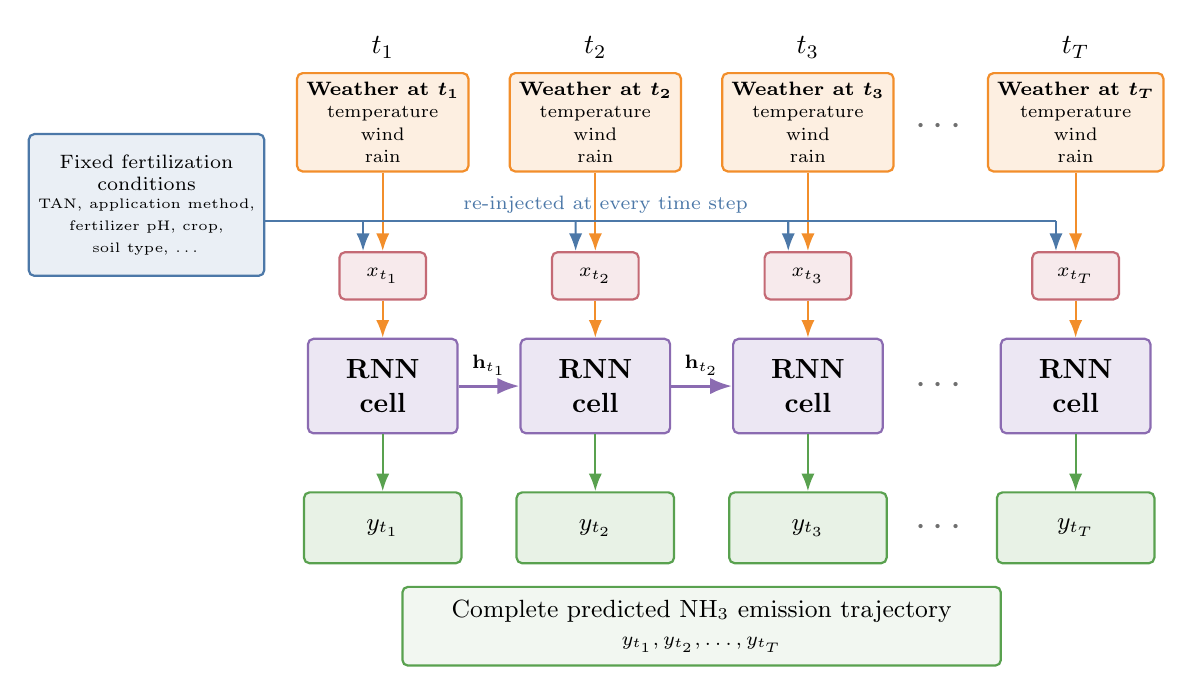
\begin{tikzpicture}[
  font=\small,
  >=Latex,
  box/.style={rounded corners=2pt, draw, line width=0.8pt,
              minimum width=25mm, minimum height=9mm, align=center},
  fixed/.style={box, draw=fixedblue, fill=fixedblue!12},
  weather/.style={box, draw=weatherorange, fill=weatherorange!14, minimum width=20mm, minimum height=8mm, font=\scriptsize},
  input/.style={box, draw=inputrose, fill=inputrose!14, minimum width=11mm, minimum height=6mm, font=\scriptsize},
  cell/.style={box, draw=rnnpurple, fill=rnnpurple!16,
               minimum width=19mm, minimum height=12mm, font=\bfseries},
  output/.style={box, draw=outputgreen, fill=outputgreen!14,
                 minimum width=20mm},
  arrow/.style={->, line width=0.75pt, draw=black!70},
  state/.style={->, line width=1.1pt, draw=rnnpurple},
  note/.style={font=\scriptsize, align=center, text=softgray},
  time/.style={font=\bfseries}
]

% Shared, time-invariant fertilization context
\node[fixed, minimum width=23mm, minimum height=18mm, font=\scriptsize] (fixed) at (-3.0,1.95)
  {Fixed fertilization\\conditions\\[-0.5mm]
   \tiny TAN, application method,\\ \tiny fertilizer pH, crop,\\ \tiny soil type, \ldots};

% The RNN is shown unrolled over four representative time steps.
\foreach \x/\lab/\i in {0/t_1/1,2.7/t_2/2,5.4/t_3/3,8.8/t_T/4}{
  \node[time] (time-\i) at (\x,3.95) {$\lab$};
  \node[weather] (weather-\i) at (\x,3.0)
    {{\bfseries Weather at \boldmath$\lab$} \\ {\normalfont\fontseries{m}\selectfont\scalebox{0.94}{temperature}} \\
     {\normalfont\fontseries{m}\selectfont\scalebox{0.94}{wind}} \\
     {\normalfont\fontseries{m}\selectfont\scalebox{0.94}{rain}}};
  \node[input] (input-\i) at (\x,1.05) {$x_{\lab}$};
  \node[cell] (rnn-\i) at (\x,-0.35) {RNN\\cell};
  \node[output] (out-\i) at (\x,-2.15)
    {$y_{\lab}$};
  \draw[arrow, draw=weatherorange] (weather-\i.south) -- (input-\i.north);
  \draw[arrow, draw=weatherorange] (input-\i) -- (rnn-\i);
  \draw[arrow, draw=outputgreen] (rnn-\i) -- (out-\i);
}

% Ellipsis indicates any number of intermediate time steps.
\node[font=\Large, text=softgray] at (7.10,-0.35) {$\cdots$};
\node[font=\Large, text=softgray] at (7.10,2.95) {$\cdots$};
\node[font=\Large, text=softgray] at (7.10,-2.15) {$\cdots$};

% The same fixed variables are injected into every cell.
\draw[draw=fixedblue, line width=0.75pt] ($(fixed.east)+(0,-0.20)$) -- (8.55,1.75);
\foreach \x/\i in {0/1,2.7/2,5.4/3,8.8/4}
  \draw[arrow, draw=fixedblue] ({\x-0.25},1.75) -- ($(input-\i.north)+(-0.25,0)$);
\node[note, text=fixedblue, anchor=west] at (0.9,1.95)
  {re-injected at every time step};

% Recurrent hidden state.
\draw[state] (rnn-1) -- node[above, font=\scriptsize] {$\mathbf{h}_{t_1}$} (rnn-2);
\draw[state] (rnn-2) -- node[above, font=\scriptsize] {$\mathbf{h}_{t_2}$} (rnn-3);

% Conceptual summary of the sequence of time-specific predictions.
\node[box, draw=outputgreen, fill=outputgreen!8,
      minimum width=76mm, minimum height=10mm]
  (trajectory) at (4.05,-3.40)
  {Complete predicted NH$_3$ emission trajectory\\[-0.3mm]
   \scriptsize $y_{t_1},y_{t_2},\ldots,
   y_{t_T}$};


\end{tikzpicture}
\end{document}

